% *********************************************************************
% © 2021-2023 Jeremy Sylvestre
%
% Permission is granted to copy, distribute and/or modify this document
% under the terms of the GNU Free Documentation License, Version 1.3 or
% any later version published by the Free Software Foundation; with no
% Invariant Sections, no Front-Cover Texts, and no Back-Cover Texts. A
% copy of the license is included in the appendix entitled “GNU Free
% Documentation License” that appears in the output document of this
% PreTeXt source code. All trademarks™ are the registered® marks of
% their respective owners.
%
% *********************************************************************

\newcommand*{\xmin}{-2.5}
\newcommand*{\xmax}{8}
\newcommand*{\ymin}{-2.5}
\newcommand*{\ymax}{8}

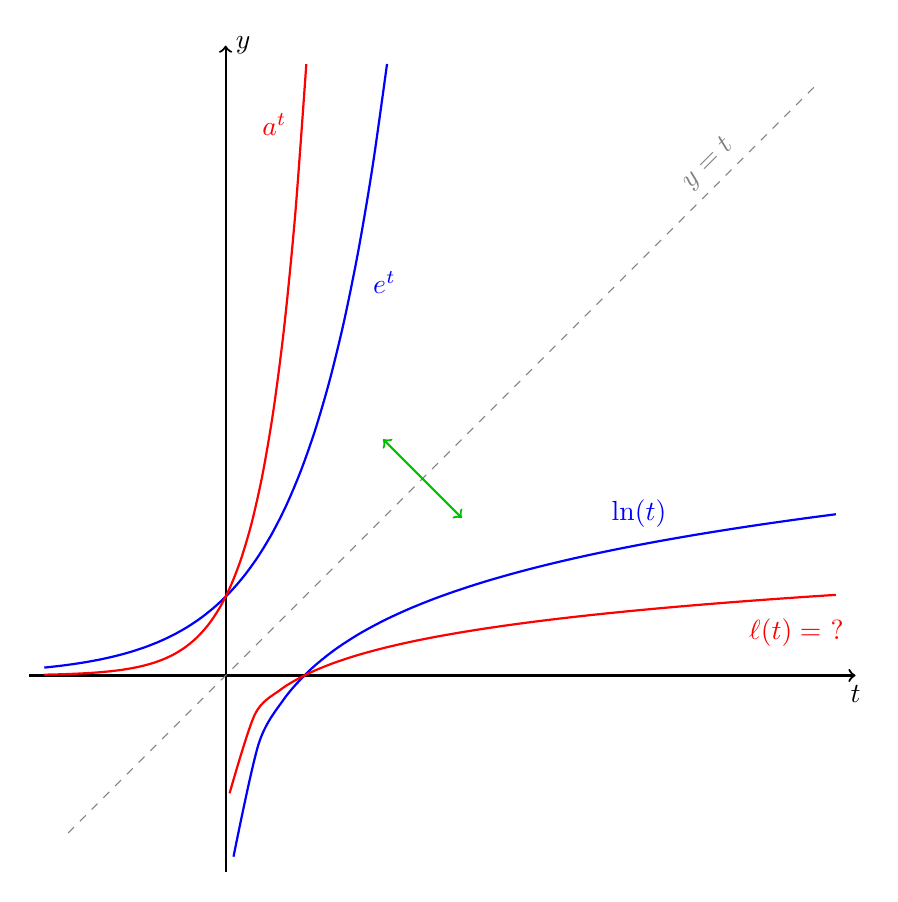
\begin{tikzpicture}
[
	closedpt/.style={circle,draw,fill,inner sep=0pt,minimum size=4pt},
	openpt/.style={circle,draw,inner sep=0pt,minimum size=4pt}
]

	% axes
	\draw[->,thick] (\xmin,0) -- (\xmax,0) node[below] {$t$};
	\draw[->,thick] (0,\ymin) -- (0,\ymax) node[right] {$y$};

	% graphs

	% exp
	\draw[thick, blue, domain=-2.303:2.05, smooth] plot (\x,{exp \x});
	\node[below right,blue] at (1.75,5.25) {$e^t$};

	% scaled exp
	\draw[thick, red, domain=-2.303:1.025, smooth] plot (\x,{exp (\x * 2)});
	\node[left,xshift=0cm,red] at (0.9,7) {$a^t$};

	% natural log
	\draw[thick, blue, domain=0.1:7.75, smooth] plot (\x,{ln \x});
	\node[above,yshift=0.1cm,blue] at (5.25,1.658) {$\ln(t)$};

	% scaled natural log
	\draw[thick, red, domain=0.05:7.75, smooth] plot (\x,{(ln \x) / 2});
	\node[below,red] at (7.25,0.85) {$\ell(t) = $ ?};

	\draw[dashed,gray,thin] (-2,-2) -- node[above,sloped,very near end] {$y = t$} (7.5,7.5);
%	\draw[<->,red] (2,3) -- node[above,sloped] {reflect} (3,2);
	\draw[thick,<->,green!75!black] (2,3) -- (3,2);

\end{tikzpicture}
